\documentclass[a4paper,11pt]{jsarticle}

\usepackage{amsmath,amsfonts}
\usepackage{amssymb}
\usepackage{bm}
\usepackage[dvipdfmx]{graphicx}
\usepackage{ascmac}
\usepackage{fancybox}
\usepackage{tikz}
\usepackage{amsthm}
\usepackage{expl3}
\usepackage{ytableau}
\usepackage{here}
\usepackage{url}
\usetikzlibrary{positioning, intersections, calc, arrows.meta,math, decorations.markings}


\theoremstyle{plain}
\newtheorem{thm}{Theorem}
\newtheorem*{thm*}{Theorem}

\theoremstyle{definition}
\newtheorem{dfn}{Definition}

\newtheorem{lem}{Lemma}

% 括弧のサイズを自動調整
\renewcommand{\(}{\left(}
\renewcommand{\)}{\right)}
\renewcommand{\[}{\left[}
\renewcommand{\]}{\right]}
\renewcommand{\{}{\left\lbrace}
\renewcommand{\}}{\right\rbrace}

\newcommand{\abs}[1]{\left| #1 \right|} % 絶対値

% 矢印
\newcommand{\Iff}{\Longleftrightarrow}
\newcommand{\To}{\Longrightarrow}
\newcommand{\ShortTo}{\Rightarrow}

% 行列
\newcommand{\pmat}[1]{\begin{pmatrix} #1 \end{pmatrix}}
\newcommand{\mat}[1]{\left( \begin{matrix} #1 \end{matrix} \right)}
\newcommand{\dmat}[1]{\left| \begin{matrix} #1 \end{matrix} \right|}

% 微分
\ExplSyntaxOn
\newcommand{\ppartial}[1]
    {
        \pd_parse:n { #1 }
    }
    \cs_new_protected:Nn \pd_parse:n
    {
    \seq_set_split:Nnn \l_tmpa_seq { , } { #1 }
    \partial \seq_use:Nn \l_tmpa_seq { \partial }
}

\newcommand{\pd}[2]{
    \frac{\partial{#1}}{\ppartial{#2}}
}
\ExplSyntaxOff

% 集合
\newcommand{\R}{\mathbb{R}}
\newcommand{\N}{\mathbb{N}}
\newcommand{\Z}{\mathbb{Z}}
\newcommand{\Q}{\mathbb{Q}}
\newcommand{\C}{\mathbb{C}}
\newcommand{\F}{\mathbb{F}}
\newcommand{\K}{\mathbb{K}}

\begin{document}

\title{RSK対応の応用とフック長公式}
\author{dragoemon}
\date{\today}
\maketitle



\ytableausetup{centertableaux}

*がついた問題は、発表時間中に出す予定の問題なので、解答は最後に載せている。

\section{フック長公式}

\begin{itembox}[l]{定義}
    ヤング図形$\lambda$とその箱$c$に対して、$c$のフックとは、
    \begin{enumerate}
        \item $c$
        \item $c$と同じ行で$c$の右側にある箱
        \item $c$と同じ列で$c$の下側にある箱
    \end{enumerate}
    を合わせた箱の集合である。
    \begin{figure}[H]
        \begin{center}
            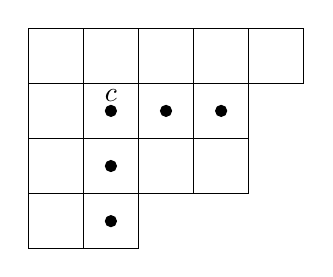
\begin{tikzpicture}[scale=0.7]
                % ヤング図形の描画
                \draw (0,0) grid (1,1);
                \draw (1,0) grid (2,1);
                \draw (2,0) grid (3,1);
                \draw (3,0) grid (4,1);
                \draw (4,0) grid (5,1);
                \draw (0,-1) grid (1,0);
                \draw (1,-1) grid (2,0);
                \draw (2,-1) grid (3,0);
                \draw (3,-1) grid (4,0);
                \draw (0,-2) grid (1,-1);
                \draw (1,-2) grid (2,-1);
                \draw (2,-2) grid (3,-1);
                \draw (3,-2) grid (4,-1);
                \draw (0,-3) grid (1,-2);
                \draw (1,-3) grid (2,-2);

                % フックの描画 (円を描く)
                \draw[fill=black] (1.5,-0.5) circle [radius=0.1] node[above]{$c$};
                \draw[fill=black] (2.5,-0.5) circle [radius=0.1];
                \draw[fill=black] (3.5,-0.5) circle [radius=0.1];
                \draw[fill=black] (1.5,-1.5) circle [radius=0.1];
                \draw[fill=black] (1.5,-2.5) circle [radius=0.1];
            \end{tikzpicture}
        \end{center}
    \end{figure}
    フック長$h(c) = h_{\lambda}(c)$とは、$c$のフックに含まれる箱の個数である。上の例では$h(c) = 5$である。
    $i$行$j$列の箱を$(i,j)$と書き、$h_{\lambda}(i,j)$で$(i,j)$のフック長を表すこともある。
\end{itembox}

数$f^\lambda$や$d_\lambda(m)$には、フック長を用いた公式がいくつか存在する。その中でも特に有名なのが次のフック長公式である。
(私が組合せ論にハマるきっかけとなった公式である。)

\begin{itembox}[l]{定理(フック長公式)}
    \begin{align*}  
        f^\lambda = \frac{|\lambda|!}{\displaystyle \prod_{c \in \lambda} h_{\lambda}(c)}
    \end{align*}
    ここで、$|\lambda|$はヤング図形$\lambda$の箱の個数であり、分母の$c$は$\lambda$の全ての箱を動く。
\end{itembox}

たとえば、ヤング図形
\begin{align*}
    (5,4,4,2) = \ydiagram[]{5,4,4,2}
\end{align*}
に対して、各箱にフック長を書き込むと、
\begin{align*}
    \begin{ytableau}
        8 & 7 & 5 & 4 & 1 \\
        6 & 5 & 3 & 2 \\
        5 & 4 & 2 & 1 \\
        2 & 1
    \end{ytableau}
\end{align*}
となるので、$(5,4,4,2)$の標準タブローの個数は
\begin{align*}
    f^{(5,4,4,2)} = \frac{15!}{8 \cdot 7 \cdot 5 \cdot 4 \cdot 1 \cdot 6 \cdot 5 \cdot 3 \cdot 2 \cdot 5 \cdot 4 \cdot 2 \cdot 1 \cdot 2 \cdot 1} = 81081
\end{align*}
である。

\begin{itembox}[l]{問題*}
    $f^{(n,n)}$をカタラン数という。$f^{(n,n)} = \frac{(2n)!}{n!(n+1)!}$をフック長公式を用いて示せ。
\end{itembox}

これからフック長公式の証明を行うのであるが、その前にフック長公式をぱっと覚える(?)方法を紹介する。

ヤング図形$\lambda \vdash n$に対して、$1$から$n$までの整数を書き込む$n!$通りの方法がある。
このうち、中身がちゃんとタブローになるのは、すべてのフックにおいてフックの角に書かれた整数がそのフックの中で最小であるときである。
フック長を$h$とすると、そうなる確率は$\frac{1}{h}$なので、もしそうなる確率が独立ならば(実際には独立ではないが)、フック長公式が成り立つ。

実はこの議論を精密化した確率論的証明が存在する。[Greene, Nijenhuis, Wilf (1979)]によるものである。
ヤング図形のある箱からスタートして、フックの中の箱をランダムに選ぶという操作を繰り返すことで、外隅に至る経路ができる。(この操作をフックウォークという。)
最初にランダムに箱を選び、そこからのフックウォークである外隅に至る確率を、すべての外隅について足したものは$1$になる。これを利用すると、フック長公式が証明できる。
詳細は、私が高校生のときに解説記事を出したので、興味があれば読んでみてほしい。:
\url{https://mathlog.info/articles/3114}

\begin{itembox}[l]{補題1}
    $\lambda = (\lambda_1, \lambda_2, \ldots, \lambda_k) \vdash n$とする。
    $l_i:= \lambda_i + k - i \quad (1 \leq i \leq k)$とする。\\
    (こうすることで、$l_1 > l_2 > \ldots > l_k \geq 0$となる。)
    このとき、次の等式が成り立つ。
    \begin{align*}
        \frac{n!}{ \displaystyle \prod_{c \in \lambda} h_{\lambda}(c)} = \frac{n! \displaystyle \prod_{i<j}(l_i-l_j)}{l_1! l_2! \cdots l_k!}
    \end{align*}
\end{itembox}

\begin{proof}
    % $i$行目の箱のフック長の積
    % \begin{align*}
    %     \prod_{j=1}^{\lambda_i} h_{\lambda}(i,j)
    % \end{align*}
    % を考える。
    \begin{align*}
        H_\lambda = \prod_{c \in \lambda} h_{\lambda}(c)
    \end{align*}
    とする。
    \begin{align*}
        H_\lambda = \frac{l_1! l_2! \cdots l_k!}{\prod_{i<j}(l_i-l_j)}
    \end{align*}
    を$k$に関する帰納法で示す。$k=1$のとき、ヤング図形は$(n)$であり、$H_\lambda = n!$であるから成立する。$k \geq 2$とする。
    $\lambda' = (\lambda_1 - \lambda_k, \lambda_2 - \lambda_k, \ldots, \lambda_{k-1} - \lambda_k), \quad \mu = (\lambda_k^{k-1})$とする。
    このとき、$\lambda$は$(\lambda_k), \mu, \lambda'$に切り分けられる。言い換えれば、$(\lambda_k) \ast \lambda' = \lambda / \mu$となる。\\
    \begin{figure}[H]
        \begin{center}
            \begin{tikzpicture}[scale=0.6]
                \draw (0,0) -- (10,0) -- (10,-1) -- (8,-1) -- (8,-2) -- (7,-2) -- (7,-3) -- (5,-3) -- (5,-4) -- (3,-4) -- (3,-5) -- (0,-5) -- (0,0);
                \draw (0,-4) -- (3,-4);
                \draw (3,0) -- (3,-4);
                \node at (1.5,-2) {$\mu$};
                \node at (5,-1.5) {$\lambda'$};
                \node at (1.5,-4.5) {$(\lambda_k)$};
                % \node at (-0.5,0.5) [above left]{$\lambda$};
            \end{tikzpicture}
        \end{center}
    \end{figure}
    したがって、
    \begin{align*}
        H_\lambda = H_{(\lambda_k)} \cdot H_{\lambda'} \cdot \prod_{c \in \mu} h_{\lambda}(c)
    \end{align*}
    である。明らかに、
    \begin{align*}
        H_{(\lambda_k)} = \lambda_k! = l_k!
    \end{align*}
    である。帰納法の仮定より、
    \begin{align*}
        H_{\lambda'} &= \frac{\displaystyle \prod_{i=1}^{k-1} (\lambda_i - \lambda_k + (k - 1) -i)!}{\displaystyle \prod_{i<j(<k)} \{(\lambda_j + (k-1) - j) - (\lambda_i + (k-1) - i)\}} \\
        &= \frac{\displaystyle \prod_{i=1}^{k-1} (l_i - l_k - 1)!}{\displaystyle \prod_{i<j(<k)} (l_i-l_j)}
    \end{align*}
    である。また、
    \begin{align*}
        \prod_{c \in \mu} h_{\lambda}(c) &= \prod_{i=1}^{k-1} \prod_{j=1}^{\lambda_k} h_{\lambda}(i,j) \\
        &= \prod_{i=1}^{k-1} \prod_{j=1}^{\lambda_k} \{(\lambda_i - j) + (k - i) + 1\} \\
        &= \prod_{i=1}^{k-1} \prod_{j=1}^{\lambda_k} (l_i + 1 - j) \\
        &= \prod_{i=1}^{k-1} \frac{l_i!}{(l_i - \lambda_k)!} \\
        &= \prod_{i=1}^{k-1} \frac{l_i!}{(l_i - l_k)!} \\
    \end{align*}
    である。以上より、
    \begin{align*}
        H_\lambda &= l_k! \cdot \frac{\displaystyle \prod_{i=1}^{k-1} (l_i - l_k - 1)!}{\displaystyle \prod_{i<j(<k)} (l_i-l_j)} \cdot \prod_{i=1}^{k-1} \frac{l_i!}{(l_i - l_k)!} \\
        &= \frac{l_1! l_2! \cdots l_k!}{\prod_{i<j}(l_i-l_j)}
    \end{align*}
    である。したがって、次の等式が成り立つ。
    \begin{align*}
        \frac{n!}{ H_{\lambda} } = \frac{n! \displaystyle \prod_{i<j}(l_i-l_j)}{l_1! l_2! \cdots l_k!}
    \end{align*}
\end{proof}


\begin{itembox}[l]{補題2}
    $f^\lambda$について次の漸化式が成り立つ。
    \begin{align*}
        f^{(\lambda_1, \lambda_2, \ldots, \lambda_k)} = \sum_{i=1}^{k} f^{(\lambda_1, \lambda_2, \ldots, \lambda_i - 1 \ldots, \lambda_{k})}
    \end{align*}
    ただし、$(\lambda_1, \lambda_2, \ldots, \lambda_i - 1 \ldots, \lambda_{k})$が分割でないとき(つまり、$\lambda_{i-1} = \lambda_i$のとき)は、$f^{(\lambda_1, \lambda_2, \ldots, \lambda_i - 1 \ldots, \lambda_{k})} = 0$とする。
\end{itembox}

\begin{proof}
    $\lambda$の標準タブローを定めることは、$n$が入る箱を一つ選び、それを取り除いた残りのヤング図形の標準タブローを定めることに他ならない。よって、
    \begin{align*}
        f^{\lambda} = \sum_{\mu} f^{\mu}
    \end{align*}
    である。ただし、$\mu$は$\lambda$から箱を一つ取り除いたヤング図形全体を動く。$\lambda$の$i$行目から箱を取り除いたものは$(\lambda_1, \ldots, \lambda_i - 1, \ldots, \lambda_k)$であるので、
    \begin{align*}
        f^{(\lambda_1, \ldots, \lambda_i, \ldots, \lambda_k)} = \sum_{i=1}^{k} f^{(\lambda_1, \ldots, \lambda_i - 1, \ldots, \lambda_k)}
    \end{align*}
\end{proof}

\begin{itembox}[l]{補題3}
    \begin{align*}
        F(l_1, l_2, \cdots, l_k) = \frac{n! \prod_{i<j}(l_i-l_j)}{l_1! l_2! \cdots l_k!}
    \end{align*}
    とする。
    \begin{align*}
        F(l_1, l_2, \cdots, l_k) = \sum_{i=1}^{k} F(l_1, l_2, \cdots, l_i - 1, \cdots, l_k)
    \end{align*}
    が成り立つ。
\end{itembox}

\begin{proof}
    \begin{align*}
        \Delta(l_1, l_2, \cdots, l_k) := \prod_{i<j}(l_i-l_j)
    \end{align*}
    とする。示すべき等式を同値変形すると、
    \begin{align*}
        & F(l_1, l_2, \cdots, l_k) = \sum_{i=1}^{k} F(l_1, l_2, \cdots, l_i - 1, \cdots, l_k) \\
        &\Iff \frac{n! \Delta(l_1, l_2, \cdots, l_k)}{l_1! l_2! \cdots l_k!} = \sum_{i=1}^{k} \frac{(n-1)! \Delta(l_1, l_2, \cdots, l_i - 1, \cdots, l_k)}{l_1! l_2! \cdots (l_i-1)! \cdots l_k!} \\
        &\Iff n \Delta(l_1, l_2, \cdots, l_k) = \sum_{i=1}^{k} l_i \Delta(l_1, l_2, \cdots, l_i - 1, \cdots, l_k) \\
    \end{align*}
    である。これは、より一般的な次の等式から導かれる。
    \begin{align}
        \(x_1+\cdots+x_k-\frac{k(k-1)}{2}t\) \cdot \Delta(x_1, x_2, \cdots, x_k) = \sum_{i=1}^{k} x_i \Delta(x_1, x_2, \cdots, x_i - t, \cdots, x_k)  \label{eq:1}
    \end{align}
    実際、$x_j = l_j (1 \leq j \leq k), t = 1$とすると、
    \begin{align*}
        x_1 + x_2 + \cdots + x_k - \frac{k(k-1)}{2}t = \sum_{j=1}^{k} (\lambda_j + k - j) - \frac{k(k-1)}{2} = n
    \end{align*}
    であるから、示すべき等式が成り立つ。したがって、(\ref{eq:1})が成り立つことを示せばよい。
    \begin{align*}
        f_t(x_1, x_2, \cdots, x_k) := \sum_{i=1}^{k} x_i \Delta(x_1, x_2, \cdots, x_i - t, \cdots, x_k)
    \end{align*}
    とする。$f_t$が交代式であることを示す。$1 \leq i < j \leq k$なる$i,j$に対し$x_i$と$x_j$を入れ替えると、
    \begin{align*}
        f_t(x_1, \cdots,x_j ,\cdots, x_i,\cdots, x_k) &= \sum_{m=1}^{k} x_m \Delta(x_1, \cdots, x_j ,\cdots, x_i,\cdots, x_m - t,\cdots, x_k) \\
        &= -\sum_{m\neq i,j} x_m \Delta(x_1, \cdots, x_m - t,\cdots, x_k)  \\
        &+ x_j \Delta(x_1, \cdots, x_j - t,\cdots, x_i,\cdots, x_k) \\
        &+ x_i \Delta(x_1, \cdots, x_j,\cdots, x_i - t,\cdots, x_k) \\
        &= -\sum_{m\neq i,j} x_m \Delta(x_1, \cdots, x_m - t,\cdots, x_k)  \\
        &- x_i \Delta(x_1, \cdots, x_i- t,\cdots, x_j,\cdots, x_k) \\
        &- x_j \Delta(x_1, \cdots, x_i,\cdots, x_j - t,\cdots, x_k) \\
        &= - f_t(x_1, \cdots,x_i ,\cdots, x_j,\cdots, x_k)
    \end{align*}
    となる。したがって、$f_t$は交代式であるから、因数定理より、
    \begin{align*}
        f_t(x_1, x_2, \cdots, x_k) = g_t(x_1,x_2,\cdots,x_k) \cdot \Delta(x_1, x_2, \cdots, x_k)
    \end{align*}
    なる対称式$g_t$が存在する。両辺の次数を比較すれば、$g_t$は$x_1, \cdots, x_k$に関して一次式であることがわかるので、
    \begin{align*}
        g_t(x_1, x_2, \cdots, x_k) = A_t (x_1 + x_2 + \cdots + x_k) + B_t
    \end{align*}
    である。$A_t,B_t$は$t$についての多項式であり、$x_1, \cdots, x_k$に依存しない。ここで、$x_i = t(k-i) \quad (1 \leq i \leq k)$を代入すると、
    \begin{align*}
        f_t(t(k-1), t(k-2), \cdots, 0) = \{A_t \cdot \frac{k(k-1)}{2}t + B_t\} \cdot \Delta(t(k-1), t(k-2), \cdots, 0)
    \end{align*}
    であり、左辺$\displaystyle \sum_{i=1}^{k} x_i \Delta(x_1, x_2, \cdots, x_i - t, \cdots, x_k)$の各項は、
    \begin{itemize}
        \item $i < k$のとき、$x_i - t = x_{i+1}$であるから、$\Delta(x_1, x_2, \cdots, x_i - t, \cdots, x_k) = 0$である。
        \item $i = k$のとき、$x_i = 0$である。
    \end{itemize}
    したがって、$f_t(t(k-1), t(k-2), \cdots, 0) = 0$である。$\Delta(t(k-1), t(k-2), \cdots, 0) \neq 0$であるから、$g_t = 0$である。よって、
    $B_t = -t \cdot A_t \cdot \frac{k(k-1)}{2}$である。以上より、
    \begin{align*}
        g_t(x_1, x_2, \cdots, x_k) = A_t \{x_1 + x_2 + \cdots + x_k - \frac{k(k-1)}{2} t \}
    \end{align*}
    を得る。次に$x_i = t(k-i+1)$を代入すると、
    \begin{align*}
        f_t(kt, (k-1)t, \cdots, 2t, t) = A_t \{\frac{k(k+1)}{2} t - \frac{k(k-1)}{2} t \} \cdot \Delta(kt, (k-1)t, \cdots, 2t, t)
    \end{align*}
    であり、左辺は$\displaystyle \sum_{i=1}^{k} x_i \Delta(x_1, x_2, \cdots, x_i - t, \cdots, x_k)$について、$i<k$のときは$\Delta(x_1, x_2, \cdots, x_i - t, \cdots, x_k) = 0$であるので、
    \begin{align*}
        f_t(kt, (k-1)t, \cdots, 2t, t) &= t \cdot \Delta(kt, (k-1)t, \cdots, 2t, 0) \\
        &= t \cdot \Delta(kt, (k-1)t, \cdots, 2t, t) \cdot \frac{\prod_{i=1}^{k-1} (t(k-i+1) - 0)}{\prod_{i=1}^{k-1} (t(k-i+1) - t)} \\
        &= t \cdot \Delta(kt, (k-1)t, \cdots, 2t, t) \cdot \frac{k!}{(k-1)!} \\
        &= kt \cdot \Delta(kt, (k-1)t, \cdots, 2t, t)
    \end{align*}
    である。$\Delta(kt, (k-1)t, \cdots, 2t, t) \neq 0$であるから、
    \begin{align*}
        kt = A_t \{\frac{k(k+1)}{2} t - \frac{k(k-1)}{2} t \}
    \end{align*}
    より、$A_t = 1$である。以上より、
    \begin{align*}
        f_t(x_1, x_2, \cdots, x_k) = \Delta(x_1, x_2, \cdots, x_k) \cdot \{x_1 + x_2 + \cdots + x_k - \frac{k(k-1)}{2} t \}
    \end{align*}
    なので、(\ref{eq:1})が成り立つ。
\end{proof}


\begin{itembox}[l]{定理(フック長公式)}
    $\lambda \vdash n$に対して、
    \begin{align*}
        f^\lambda = \frac{n!}{\prod_{c \in \lambda} h_{\lambda}(c)}
    \end{align*}
\end{itembox}

\begin{proof}
    $n$についての帰納法で示す。$n=1$のときは両辺は$1$であるから成立する。$n \geq 2$とする。補題1,2,3より、
    \begin{align*}
        f^{(\lambda_1, \lambda_2, \ldots, \lambda_k)} &= \sum_{i=1}^{k} f^{(\lambda_1, \lambda_2, \ldots, \lambda_i - 1 \ldots, \lambda_{k})} \\
        &= \sum_{i=1}^{k} \frac{(n-1)!}{H_{(\lambda_1, \cdots, \lambda_i - 1, \cdots, \lambda_k)}} \\
        &= \sum_{i=1}^{k} F(l_1, l_2, \cdots, l_i - 1,\cdots  l_k) \\
        &= F(l_1, l_2, \cdots, l_k) \\
        &= \frac{n!}{H_{(\lambda_1, \cdots, \lambda_k)}} \\
    \end{align*}
    である。したがって、フック長公式が成り立つ。
\end{proof}


数$d_\lambda(m)$にもフック長公式が存在する。証明は6章の演習問題42にて行う。
\begin{itembox}[l]{定理}
    \begin{align*}
        d_\lambda(m) = \prod_{(i,j) \in \lambda} \frac{m + j - i}{h_{\lambda}(i,j)}
    \end{align*}
\end{itembox}

\newpage
\section{演習問題の解答}



\begin{itembox}[l]{問題19}
    任意の$k \geq 2$に対して、次の等式が成り立つことを示せ。
    \begin{align*}
        \sum \frac{\prod_{i<j}(l_i-l_j)^2}{l_1!^2 l_2!^2 \cdots l_k!^2} = 1
    \end{align*}
    ただし、和はすべての非負整数の組$l_1, l_2, \ldots, l_k$であって$l_1 + l_2 + \cdots + l_k = \frac{k(k+1)}{2}$を満たすものを取る。
\end{itembox}

\begin{proof}
    分子$\prod_{i<j}(l_i-l_j)^2$は$l_1, \cdots, l_k$について対称であり、$l_i = l_j$なる$i<j$が存在するとき$0$であることに注意すれば、
    \begin{align*}
        \sum \frac{\prod_{i<j}(l_i-l_j)^2}{l_1!^2 l_2!^2 \cdots l_k!^2} &= \sum{}^{'} \frac{k! \prod_{i<j}(l_i-l_j)^2}{l_1!^2 l_2!^2 \cdots l_k!^2}
    \end{align*}
    である。ここで、$\sum{}^{'}$は$l_1 > l_2 > \cdots > l_k \geq 0, l_1 + l_2 + \cdots + l_k = \frac{k(k+1)}{2}$を満たす非負整数の組$l_1, \cdots, l_k$についての和である。
    また、フック長公式の変形(補題1)とロビンソン対応より、
    \begin{align*}
        \sum{}^{'} \frac{k!^2 \prod_{i<j}(l_i-l_j)^2}{l_1!^2 l_2!^2 \cdots l_k!^2} &= \sum_{\lambda \vdash k} (f^{\lambda})^2 = k!
    \end{align*}
    である。したがって、
    \begin{align*}
        \sum \frac{\prod_{i<j}(l_i-l_j)^2}{l_1!^2 l_2!^2 \cdots l_k!^2} = 1
    \end{align*}
\end{proof}

\begin{itembox}[l]{問題20}
    % \begin{enumerate}
        (1) $n$次置換群$S_n$の元で、最大増加列の長さが$l$、最大減少列の長さが$k$であるものの数は$\sum (f^{\lambda})^2$であることを示せ。ただし、$\lambda$は$n$の分割であり、$k$個の行と$l$個の列からなるものをすべて動く。\\
        (2*) $S_{21}$の元で、最大増加列の長さが$15$、最大減少列の長さが$4$であるものの数を求めよ。
    % \end{enumerate}
\end{itembox}

\subitem (1)
ロビンソン対応により、$n$次置換群$S_n$の元と同じ形$\lambda \vdash n$の標準タブローの組$(P,Q)$が1対1に対応する。ここで最大増加列の長さは$\lambda$の行数、最大減少列の長さは$\lambda$の列数である。したがって、等式が成り立つ。

\subitem (2)
最後に載せてある。


\begin{itembox}[l]{問題21}
    $m, n$を$m \leq n \leq 2m$なる正の整数とする。$1$と$2$からなる長さ$n$の列で、最大非減少部分列の長さが$m$であるものの数を求めよ。
\end{itembox}


ロビンソン・シェンステッド対応によって、求める数は
\begin{align*}
    \sum f^{\lambda} \cdot d_{\lambda}(2)
\end{align*}
である。ここで、$\lambda$は列数が$m$である$n$の分割すべてを動く。ここで$\lambda$が$3$行以上のときは$d_{\lambda}(2) = 0$であるから、
$\lambda$が2行以下であるときを考えればよいが、この条件を満たす分割は$\lambda = (m,n-m)$のみであるから、求めるべき数は
\begin{align*}
    f^{(m,n-m)} \cdot d_{(m,n-m)}(2)
\end{align*}
である。フック長公式より、
\begin{align*}
    f^{(m,n-m)} \cdot d_{(m,n-m)}(2) = \frac{n!}{H_{(m,n-m)}} \cdot \frac{\prod_{(i,j) \in (m,n-m)} (2-i+j)}{H_{(m,n-m)}}
\end{align*}
である。箱$i,j$に$2-i+j$を書き込むと、
\begin{align*}
    \ytableausetup{boxsize=3em}
    \begin{ytableau}
        2 & 3 & \cdots & \cdots & \cdots & \cdots & m+1 \\
        1 & 2 & \cdots & n-m
    \end{ytableau}
    \ytableausetup{boxsize=1.5em}
\end{align*}
であるから、
\begin{align*}
    \prod_{(i,j) \in (m,n-m)} (2-i+j) = (n-m)! \cdot (m+1)!
\end{align*}
である。また、各箱にフック長を書き込むと、
\begin{align*}
    \ytableausetup{boxsize=3.3em}
    \begin{ytableau}
        m+1 & m & \cdots & \scriptstyle 2m-n+2 & \scriptstyle 2m-n & \cdots & 1 \\
        n-m & \scriptstyle n-m-1 & \cdots & 1
    \end{ytableau}
    \ytableausetup{boxsize=1.5em}
\end{align*}
であるから、
\begin{align*}
    H_{(m,n-m)} = \frac{(m+1)! (n-m)!}{2m-n+1}
\end{align*}
である。以上より、求める数は
\begin{align*}
    & \frac{n!(2m-n+1)}{(m+1)!(n-m)!} \cdot \frac{(n-m)! \cdot (m+1)! \cdot (2m-n+1)}{(m+1)!(n-m)!} \\
    &= \frac{n!(2m-n+1)^2}{(m+1)!(n-m)!}
\end{align*}


\begin{itembox}[l]{問題22}
    次の等式を示せ。
    \begin{align*}
        \prod_{i=1}^{\infty} \frac{1}{1-x_i} \prod_{1 \leq i < j \leq m} \frac{1}{1-x_i x_j} = \sum_{\lambda} s_{\lambda}(x_1, x_2, \ldots, x_m)
    \end{align*}
\end{itembox}

\begin{proof}
    ロビンソン・シェンステッド・クヌース対応において、タブロー対$(P,P)$は対称行列と一対一に対応する。したがって、
    \begin{align*}
        \sum_{\lambda} s_{\lambda}(x_1, x_2, \ldots, x_m) &= \sum_{P} x^P \\
        &= \sum_{A = A^{\top}} \prod_{i,j} x_i^{a_{ij}} \\
        &= \sum_{A = A^{\top}} \prod_{i=1}^{m} x_i^{a_{ii}} \prod_{1 \leq i < j \leq m} x_i^{a_{ij}} x_j^{a_{ji}} \\
        &= \sum_{A = A^{\top}} \prod_{i=1}^{m} x_i^{a_{ii}} \prod_{1 \leq i < j \leq m} (x_i x_j)^{a_{ij}} \\
        &= \prod_{i=1}^{m} \sum_{a_{ii}=0}^{\infty} x_i^{a_{ii}} \prod_{1 \leq i < j \leq m} \sum_{a_{ij}=0}^{\infty} (x_i x_j)^{a_{ij}} \\
        &= \prod_{i=1}^{m} \frac{1}{1-x_i} \prod_{1 \leq i < j \leq m} \frac{1}{1-x_i x_j}
    \end{align*}
\end{proof}

\begin{itembox}[l]{問題23}
    $S$を正整数の集合、$k$を整数とする。$S$の元からなるタブローで、書き込まれたすべての数字の和が$k$であるものの数は、次のべき級数の$t^k$の係数であることを示せ。
    \begin{align*}
        \prod_{a \in S} \frac{1}{1-t^a} \prod_{a<b, a,b \in S} \frac{1}{1-t^{a+b}}
    \end{align*}
\end{itembox}

\begin{proof}
    $S$が無限集合の場合は、$S\cap [k]$を改めて$S$とすれば、有限集合の場合に帰着できる。(このとき$t^k$の係数は変わらない)
    $S=\{a_1, a_2, \ldots, a_m\} \quad (a_1 < a_2 < \cdots < a_m)$とする。
    \begin{align*}
        \prod_{i=1}^{\infty} \frac{1}{1-x_i} \prod_{1 \leq i < j \leq m} \frac{1}{1-x_i x_j} = \sum_{\lambda} s_{\lambda}(x_1, x_2, \ldots, x_m)
    \end{align*}
    であった。$x_i = t^{a_i}$とする。このとき、$a_i$を$n_i$回$(1\leq i \leq n)$使うタブロー$P$について、$x^P = t^{n_1 a_1 + n_2 a_2 + \cdots + n_m a_m} = t^{\text{($P$に書き込まれた数字の和)}}$
    であるから、
    \begin{align*}
        \prod_{i=1}^{m} \frac{1}{1-t^{a_i}} \prod_{1 \leq i < j \leq m} \frac{1}{1-t^{a_i + a_j}} &= \sum_{P} t^{\text{($P$に書き込まれた数字の和)}} \\
        &= \sum_{k\in \Z} t^k \cdot \sharp \{ P \mid \text{($P$に書き込まれた数字の和)} = k \}
    \end{align*}
    である。したがって、題意は示された。
\end{proof}

\begin{itembox}[l]{問題24}
    $T$を形$\lambda$のタブローとする。$w(T)$とクヌース同値なタブローの個数がちょうど$f^{\lambda}$であることを示せ。
\end{itembox}

\begin{proof}
    ロビンソン・シェンステッド対応より、$w(T)$とクヌース同値なワード$w$とタブローの組$(T,Q)$であって$Q$が形$\lambda$の標準タブローであるものとの間に一対一対応がある。よって、$w(T)$とクヌース同値なタブローの個数は$f^{\lambda}$個である。
\end{proof}

\begin{itembox}[l]{問題25}
    $n$の置換$w$に対して、その上下列とは$n-1$個の$+$と$-$の列で$w$の増減を表したものである。すなわち、
    その$i$番目は$v_i < v_{i+1}$のとき$+$、$v_i > v_{i+1}$のとき$-$とする。このとき、$Q(w)$から$w$の上下列を復元できることを示せ。
\end{itembox}

\begin{proof}
    行バンプ補題より、$Q(w)$において$i+1$が$i$のnEにあるとき$+$、Swにあるとき$-$とすれば、$w$の上下列が復元できる。
\end{proof}

\newpage
\section{123-avoiding permutation}

ここからは本には載っていないが、4章の内容を使って私が独自に考えた話題について述べる。
この節の目標は、次の定理を証明することである。

\begin{itembox}[l]{定理}
    長さ$3$の増加部分列を持たない置換のことを123-avoiding permutationという。$n$次の置換のうち、123-avoiding permutationの個数はカタラン数$\displaystyle \frac{(2n)!}{n!(n+1)!}$である。
\end{itembox}

これの最も直感的な証明は、次のようなものである: $\sigma \in S_n$に対し、対応するDyckパスを次のように定める。$n\times n$のマス目を用意し、$i=1,2,\cdots,n$に対し$(i,\sigma(i))$を黒で塗りつぶす。
黒で塗りつぶされたマス目がすべてパスの右側にくるように、なるべく右側にパスを引く。例えば、置換$(5,3,2,6,4,1)$に対応するDyckパスは次のようになる。\\
\begin{figure}[H]
    \begin{center}
        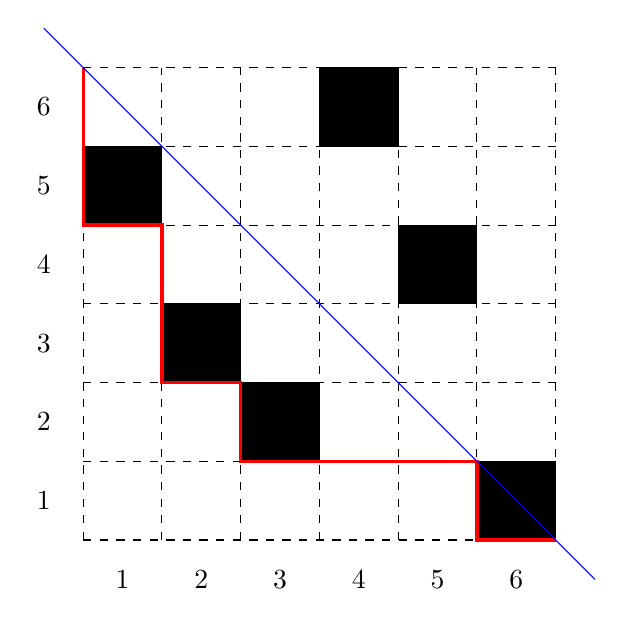
\begin{tikzpicture}
            \draw[dashed] (0,0) grid (6,6);
            \filldraw[black] (0,4) rectangle (1,5);
            \filldraw[black] (1,2) rectangle (2,3);
            \filldraw[black] (2,1) rectangle (3,2);
            \filldraw[black] (3,5) rectangle (4,6);
            \filldraw[black] (4,3) rectangle (5,4);
            \filldraw[black] (5,0) rectangle (6,1);

            %パスを書く
            \draw[red, very thick] (0,6) -- (0,4) -- (1,4) -- (1,2) -- (2,2) -- (2,1) -- (5,1) -- (5,0) -- (6,0);

            %数字を書く
            \node at (-0.5,0.5) {1};
            \node at (-0.5,1.5) {2};
            \node at (-0.5,2.5) {3};
            \node at (-0.5,3.5) {4};
            \node at (-0.5,4.5) {5};
            \node at (-0.5,5.5) {6};

            \node at (0.5,-0.5) {1};
            \node at (1.5,-0.5) {2};
            \node at (2.5,-0.5) {3};
            \node at (3.5,-0.5) {4};
            \node at (4.5,-0.5) {5};
            \node at (5.5,-0.5) {6};

            \draw[blue] (-0.5,6.5) -- (6.5,-0.5);
        \end{tikzpicture}
    \end{center}
\end{figure}
このとき、パスはDyckパスになり、これが$S_n$の元とDyckパスの間の全単射を与える。

この方法は直感的であるが、厳密に証明を補おうとすると難しい。一方で、RSK対応とフック長公式を用いて、愚直に個数を求めることもできる。
証明の第一段階を問題として示す。
\begin{itembox}[l]{問題*}
    $n$次の123-avoiding permutationの個数は
    \begin{align*}
        \sum_{k=0}^{\lfloor n/2 \rfloor} \(\frac{n! (n-2k+1)}{(n-k+1)! k!}\)^2
    \end{align*}   
    であることを示せ。
\end{itembox}

これを使えばあとはヤング図形とは関係ない。ただの計算である。

\begin{itembox}[l]{定理}
    $n$次の123-avoiding permutationの個数はカタラン数$\displaystyle \frac{(2n)!}{n!(n+1)!}$である。
\end{itembox}


\begin{proof}
    \begin{align*}
        \sum_{k=0}^{\lfloor n/2 \rfloor} \(\frac{n! (n-2k+1)}{(n-k+1)! k!}\)^2 = \frac{1}{(n+1)^2} \sum_{k=0}^{\lfloor n/2 \rfloor} (n-2k+1)^2 \pmat{n+1 \\ k}^2
    \end{align*}
    である。ここで、
    \begin{align*}
        a(n,k) := (n-2k+1) \pmat{n+1 \\ k}
    \end{align*}
    に対し、変数変換$k \mapsto n+1-k$を行うと、
    \begin{align*}
        a(n,n+1-k) = (n-2(n+1-k)+1) \pmat{n+1 \\ n+1-k} = - a(n,k)
    \end{align*}
    である。したがって、
    \begin{align*}
        \sum_{k=0}^{\lfloor n/2 \rfloor} a(n,k)^2 = \frac{1}{2} \sum_{k=0}^{n+1} a(n,k)^2
    \end{align*}
    である。また、
    \begin{align*}
        f_n(x) = \sum_{k=0}^{n+1} a(n,k) x^k
    \end{align*}
    とすると、
    \begin{align*}
        f_n(x)^2 = \sum_{m=0}^{2n+2}\( \sum_{k=0}^{m} a(n,k) a(n,m-k)\) x^m
    \end{align*}
    であるから、$f_n(x)^2$の$x^{n+1}$の係数は$\displaystyle \sum_{k=0}^{n+1} a(n,k) a(n,n+1-k) = - \sum_{k=0}^{n+1} a(n,k)^2$である。
    \begin{align*}
        f_n(x) &= \sum_{k=0}^{n+1} a(n,k) x^k \\
        &= \sum_{k=0}^{n+1} (n-2k+1) \pmat{n+1 \\ k} x^k \\
        &= (n+1) \sum_{k=0}^{n+1} \pmat{n+1 \\ k} x^k - 2 \sum_{k=0}^{n+1} k \pmat{n+1 \\ k} x^k \\
        &= (n+1) (1+x)^{n+1} - 2(n+1) \sum_{k=1}^{n+1} \pmat{n \\ k-1} x^k \\
        &= (n+1) (1+x)^{n+1} - 2(n+1)  (1+x)^{n} \\
        &= (n+1) (1+x)^{n} (x-1)
    \end{align*}
    であるから、
    \begin{align*}
        f_n(x)^2 = (n+1)^2 (1+x)^{2n} (x-1)^2
    \end{align*}
    である。これの$x^{n+1}$の係数は
    \begin{align*}
        & (n+1)^2 \cdot \{ \pmat{2n \\ n-1} -2 \pmat{2n \\ n} + \pmat{2n \\ n+1}\} \\
        &= (n+1)^2 \cdot \{ \frac{2n}{n+1}\pmat{2n \\ n} - 2\pmat{2n \\ n}\} \\
        &= - 2(n+1) \pmat{2n \\ n}
    \end{align*}
    であるので、
    \begin{align*}
        \frac{1}{2(n+1)^2} \sum_{k=0}^{n+1} a(n,k)^2 &= -\frac{1}{2(n+1)^2} \{- 2(n+1) \pmat{2n \\ n}\}  \\
        &= \frac{1}{n+1} \pmat{2n \\ n} \\
        &= \frac{(2n)!}{n!(n+1)!}
    \end{align*}
    以上より、長さ$3$の増加部分列を持たない$n$の置換の個数は$\displaystyle \frac{(2n)!}{n!(n+1)!}$である。
\end{proof}

私は現在、この定理の結果を一般化することを試みている。すなわち、正の整数$n,k$に対して、長さ$k+1$の増加部分列を持たない$n$の置換の個数を求めることである。
閉じた式での一般項は見つかっていないが、次のような公式がRSK対応とフック長公式から直ちに導かれる。

\begin{itembox}[l]{定理}
    長さ$k+1$の増加部分列を持たない$n$の置換の個数は$m := n + \frac{k(k-1)}{2}$として、
    \begin{align*}
        \frac{n!^2}{k! m!^2} \sum_{l_1+l_2+\cdots+l_k = m} \( \frac{m!}{l_1! l_2! \cdots l_k!} \Delta(l_1, l_2, \cdots, l_k) \)^2
    \end{align*}
    である。ただし、$\Delta(l_1, l_2, \cdots, l_k) := \prod_{i<j} (l_i - l_j)$であり、和は$l_1, l_2, \ldots, l_k$が非負整数であって$l_1 + l_2 + \cdots + l_k = m$を満たすものをすべて取る。
\end{itembox}

すなわち、${(\text{多項係数} \times \text{差積})}^2$の和を求めることに帰着される。

\begin{proof}
    ロビンソン対応より、$n$の置換の中で長さ$k+1$の増加部分列を持たないものは、行数が$k$以下である$n$の分割$\lambda$を形にもつ標準タブローの組$(P,Q)$と一対一に対応する。$\lambda = (\lambda_1, \lambda_2, \ldots, \lambda_k)$とすれば、
    \begin{align*}
        \sum_{\substack{\lambda_1 \geq \lambda_2 \geq \cdots \geq \lambda_k \geq 0 \\ \lambda_1 + \cdots + \lambda_k = n}} (f^{(\lambda_1, \lambda_2, \ldots, \lambda_k)})^2
    \end{align*}
    である。フック長公式の別表現より、$l = (l_1, l_2, \ldots, l_k)$を$l_i = \lambda_i + k - i$で定めると、
    \begin{align*}
        f^{(\lambda_1, \lambda_2, \ldots, \lambda_k)} = \frac{n!}{l_1! l_2! \cdots l_k!} \Delta(l_1, l_2, \cdots, l_k)
    \end{align*}
    である。したがって、求める数は
    \begin{align*}
        \sum_{\substack{l_1 > l_2 > \cdots >l_k \geq 0 \\l_1+\cdots+l_k = m}} \( \frac{n!}{l_1! l_2! \cdots l_k!} \Delta(l_1, l_2, \cdots, l_k) \)^2
    \end{align*}
    である。ここで、シグマの中身$\( \frac{m!}{l_1! l_2! \cdots l_k!} \Delta(l_1, l_2, \cdots, l_k) \)^2$は$l_1, l_2, \ldots, l_k$についての対称式であり、$l_i = l_j$なる$i < j$が存在するとき$0$であることに注意すれば、次のように変形できる。
    \begin{align*}
        \frac{1}{k!} \sum_{l_1+l_2+\cdots+l_k = m} \( \frac{n!}{l_1! l_2! \cdots l_k!} \Delta(l_1, l_2, \cdots, l_k) \)^2
    \end{align*}
    したがって、定理が示された。
\end{proof}

\newpage
\section{問題の解答}

\begin{itembox}[l]{問題}
    $f^{(n,n)}$をカタラン数という。$f^{(n,n)} = \displaystyle \frac{(2n)!}{n!(n+1)!}$をフック長公式を用いて示せ
\end{itembox}

\begin{proof}
    $(n,n)$にフック長を書き込むと、
    \begin{align*}
        \ytableausetup{boxsize=2.5em}
        \begin{ytableau}
            \scriptstyle n+1 & n & \cdots & 3 & 2 \\
            n & n-1 & \cdots & 2 & 1
        \end{ytableau}
        \ytableausetup{boxsize=1.5em}
    \end{align*}
    となる。よって、フック長の積は$n!(n+1)!$であるから、
    \begin{align*}
        f^{(n,n)} = \frac{(2n)!}{n!(n+1)!}
    \end{align*}
\end{proof}

\newpage

\begin{itembox}[l]{問題20(2)}
    $S_21$の元で、最大増加列の長さが$15$、最大減少列の長さが$4$であるものの数を求めよ。
\end{itembox}

$21$の分割のうち、$15$個の行と$4$個の列からなるものは$(15,1,1,1)$に3つの箱を加えてできるヤング図形であって、次の3通りがある。
\begin{enumerate}
    \item $\lambda^{(1)} = (15,4,1,1) = \ydiagram{15,4,1,1}$
    \item $\lambda^{(2)} = (15,3,2,1) = \ydiagram{15,3,2,1}$
    \item $\lambda^{(1)} = (15,2,2,2) = \ydiagram{15,2,2,2}$
\end{enumerate}

それぞれ、$l_i = \lambda_i + 4 - i$を計算すると、
\begin{align*}
    l^{(1)} &= (18,6,2,1) \\
    l^{(2)} &= (18,5,3,1) \\
    l^{(3)} &= (18,4,3,2) \\
\end{align*}
であるから、
\begin{align*}
    f^{(15,4,1,1)} &= \frac{21!(18-6)(18-2)(18-1)(6-2)(6-1)(2-1)}{18!6!2!1!} = 361760 \\
    f^{(15,3,2,1)} &= \frac{21!(18-5)(18-3)(18-1)(5-3)(5-1)(3-1)}{18!5!3!1!} = 587860 \\
    f^{(15,2,2,2)} &= \frac{21!(18-4)(18-3)(18-2)(4-3)(4-2)(3-2)}{18!4!3!2!} = 186200 
\end{align*}
であるから、求める数は$361760^2 + 587860^2 + 186200^2 = 511120117200$である。
\newpage

\begin{itembox}[l]{問題}
    $n$次の123-avoiding permutationの個数は
    \begin{align*}
        \sum_{k=0}^{\lfloor n/2 \rfloor} \(\frac{n! (n-2k+1)}{(n-k+1)! k!}\)^2
    \end{align*}   
    であることを示せ。
\end{itembox}

\begin{proof}
    ロビンソン対応より、$n$の置換の中で長さ$3$の増加部分列を持たないものは、行数が$2$以下である$n$の分割$\lambda$を形にもつ標準タブローの組$(P,Q)$と一対一に対応する。$P$の2行目の列数を$k$とすると、$P$の1行目の列数は$n-k$であり、$k$の動く範囲は$0 \leq k \leq \lfloor n/2 \rfloor$である。したがって、求める数は
    \begin{align*}
        \sum_{k=0}^{\lfloor n/2 \rfloor} (f^{(n-k,k)})^2
    \end{align*}
    である。フック長公式より、
    \begin{align*}
        f^{(n-k,k)} = \frac{n!}{H_{(n-k,k)}}
    \end{align*}
    である。分割$(n-k,k)$にフック長を書き込むと、
    \begin{align*}
        \ytableausetup{boxsize=3em}
        \begin{ytableau}
            \scriptstyle n-k+1 & \scriptstyle n-k & \cdots & \scriptstyle n-2k+2 & \scriptstyle n-2k & \cdots & 1 \\
            k & k-1 & \cdots & 1
        \end{ytableau}
        \ytableausetup{boxsize=1.5em}
    \end{align*}
    であるから、
    \begin{align*}
        H_{(n-k,k)} = \frac{(n-k+1)! k!}{n-2k+1}
    \end{align*}
    である。したがって、求める数は
    \begin{align*}
        \sum_{k=0}^{\lfloor n/2 \rfloor} \(\frac{n! (n-2k+1)}{(n-k+1)! k!}\)^2
    \end{align*}
\end{proof}



\end{document}